%% FullCourse_10Lecs -- Lecture 1, Topic 1.1: Intro to Quant Macro + Dynamic Programming Foundations
%% Source: ./archive_pre_split/Lec01_Quant_Macro.tex (sections 1-2)
%% Pass A mechanical split (verbatim content preserved).

%% Shared preamble for the FullCourse_10Lecs topic decks.
%%
%% Each topic .tex \input's this file, then defines its own \title, \date
%% override (if any), \graphicspath, and \begin{document}.
%%
%% Reconstructed verbatim from the inlined copy preserved in
%% Lec10_Case_Studies/Lec10_T8_Case6_DeepRamsey.tex (lines 23-190), which is
%% explicitly annotated there as "from ../shared_preamble.tex, copied verbatim".
%% Base preamble matches MiniCourse_8hr/Slides/shared_preamble.tex; this version
%% additionally provides \sectiondivider, the conceptbox/cautionbox/examplebox/
%% takeawaybox tcolorboxes, and \compacttables used across the split decks.

\documentclass[10pt,english,aspectratio=169]{beamer}

\usepackage{ae,aecompl}
\usepackage[T1]{fontenc}
\usepackage{textcomp}
\usepackage[utf8]{inputenc}
\usepackage{babel}
\usepackage{datetime2}

\setcounter{secnumdepth}{3}
\setcounter{tocdepth}{3}

\usepackage{amsmath, amssymb, amsthm, graphicx}
\usepackage{booktabs, multirow}
\usepackage{tikz}
\usepackage{pgfplots}
\pgfplotsset{compat=1.16}
\usepackage[most]{tcolorbox}
\tcbuselibrary{skins, breakable, theorems}
\usepackage{listings}
\usepackage{xcolor}

\lstset{
  basicstyle=\ttfamily\small,
  keywordstyle=\color{blue!80!black}\bfseries,
  commentstyle=\color{green!50!black}\itshape,
  stringstyle=\color{orange!80!black},
  backgroundcolor=\color{gray!8},
  frame=single,
  rulecolor=\color{gray!40},
  breaklines=true,
  showstringspaces=false,
  numbers=none,
}

\lstdefinestyle{pythonstyle}{
    language=Python,
    basicstyle=\ttfamily\footnotesize,
    keywordstyle=\color{blue!80!black}\bfseries,
    commentstyle=\color{green!50!black}\itshape,
    stringstyle=\color{orange!80!black},
    frame=single,
    breaklines=true,
    showstringspaces=false,
    numbers=left,
    numbersep=5pt,
    numberstyle=\tiny\color{gray},
    backgroundcolor=\color{gray!8},
    rulecolor=\color{gray!40}
}

\ifx\hypersetup\undefined
  \AtBeginDocument{%
    \hypersetup{bookmarks=false,breaklinks=true,pdfborder={0 0 0},colorlinks=true,
      linkcolor=DarkText,urlcolor=RedTitle}%
  }
\else
  \hypersetup{bookmarks=false,breaklinks=true,pdfborder={0 0 0},colorlinks=true,
    linkcolor=DarkText,urlcolor=RedTitle}%
\fi

\makeatletter
\newcommand\makebeamertitle{%
  \begin{frame}[plain]
    \vspace*{1.0cm}
    \centering
    {\usebeamerfont{title}\usebeamercolor[fg]{title}\inserttitle\par}
    \vspace{1.0cm}
    {\usebeamerfont{author}\usebeamercolor[fg]{author}\insertauthor\par}
    \vspace{0.2cm}
    {\usebeamerfont{date}\usebeamercolor[fg]{date}\insertdate\par}
  \end{frame}}%
\AtBeginDocument{%
  \let\origtableofcontents=\tableofcontents
  \def\tableofcontents{\@ifnextchar[{\origtableofcontents}{\gobbletableofcontents}}
  \def\gobbletableofcontents#1{\origtableofcontents}%
}

\usetheme{metropolis}
\usefonttheme{professionalfonts}

\definecolor{LightGray}{RGB}{230,230,230}
\definecolor{RedTitle}{RGB}{0,0,200}
\definecolor{VeryLightGray}{RGB}{245,245,245}
\definecolor{DarkText}{RGB}{0,0,0}

\setbeamercolor{background canvas}{bg=white}
\setbeamercolor{title}{fg=RedTitle}
\setbeamercolor{author}{fg=DarkText}
\setbeamercolor{date}{fg=DarkText}
\setbeamercolor{frametitle}{bg=VeryLightGray,fg=DarkText}
\setbeamercolor{normal text}{fg=DarkText}
\setbeamerfont{title}{size=\large}

\setbeamersize{text margin left=5mm, text margin right=5mm}
\addtobeamertemplate{frametitle}{}{\vspace{-0.5em}}
\newcommand{\reducevspace}{\vspace{-0.5cm}}

% Shared section divider and box styles for split topic decks.
\newcommand{\sectiondivider}[2]{%
\begin{frame}[plain,noframenumbering]
\begin{center}
\vfill
{\Large\textbf{#1}\par}
\vspace{0.35cm}
{\normalsize #2\par}
\vfill
\end{center}
\end{frame}
}

\newtcolorbox{conceptbox}[1][]{
  colback=blue!3,
  colframe=RedTitle!55,
  boxrule=0.35mm,
  arc=1mm,
  left=2mm,
  right=2mm,
  top=1mm,
  bottom=1mm,
  #1
}
\newtcolorbox{cautionbox}[1][]{
  colback=red!3,
  colframe=red!50!black,
  boxrule=0.35mm,
  arc=1mm,
  left=2mm,
  right=2mm,
  top=1mm,
  bottom=1mm,
  #1
}
\newtcolorbox{examplebox}[1][]{
  colback=green!3,
  colframe=green!45!black,
  boxrule=0.35mm,
  arc=1mm,
  left=2mm,
  right=2mm,
  top=1mm,
  bottom=1mm,
  #1
}
\newtcolorbox{takeawaybox}[1][]{
  colback=VeryLightGray,
  colframe=RedTitle!55,
  boxrule=0.35mm,
  arc=1mm,
  left=2mm,
  right=2mm,
  top=1mm,
  bottom=1mm,
  #1
}
\newcommand{\compacttables}{\renewcommand{\arraystretch}{1.15}}

\setbeamertemplate{navigation symbols}{}
\setbeamertemplate{footline}{%
  \hfill%
  \usebeamercolor[fg]{page number in head/foot}%
  \usebeamerfont{page number in head/foot}%
  \insertframenumber\,/\,\inserttotalframenumber\kern1em\vskip2pt%
}

\makeatother

\author{Zhigang Feng}
% "date with time": compile timestamp so each build is identifiable.
\date{\today\ \DTMcurrenttime}


\graphicspath{{./pic/}{../../FullCourse_10Lecs/Lec01_Quant_Macro/pic/}{../}}

\title[AI for Econ Research]{AI for Economic Research: Dynamic Models, Language, and Agents\\
Lecture 1.1: Introduction to Quantitative Macro \& Dynamic Programming}

\begin{document}

\makebeamertitle

%=============================================================================
\begin{frame}{Topic 1.1 Agenda}
\begin{enumerate}
  \item \textbf{What is Quantitative Macroeconomics?}
  \medskip
  \item \textbf{Dynamic Programming Foundations}
\end{enumerate}
\end{frame}

%=============================================================================
\section{What is Quantitative Macroeconomics?}

\begin{frame}{What is Quantitative Macroeconomics?}
\begin{itemize}
\item A field that uses numerical methods and computational tools to solve and analyze macroeconomic models, providing precise, quantitative answers to economic questions.

\medskip
\item \textbf{The Methodological Triad:}
\begin{enumerate}
    \item \emph{Theory:} Economic models with microfoundations
    \item \emph{Data:} Calibration and estimation
    \item \emph{Computation:} Numerical solution methods
\end{enumerate}

\medskip
\item \textbf{Core Techniques:}
\begin{itemize}
    \item Dynamic programming and optimal control
    \item Numerical optimization and root-finding
    \item Monte Carlo simulation
\end{itemize}

\medskip
\item \textbf{This Course:} Adding machine learning to the toolkit---neural networks, stochastic optimization, and deep reinforcement learning.
\end{itemize}
\end{frame}

\begin{frame}{What is Quantitative Macroeconomics?}
\begin{center}
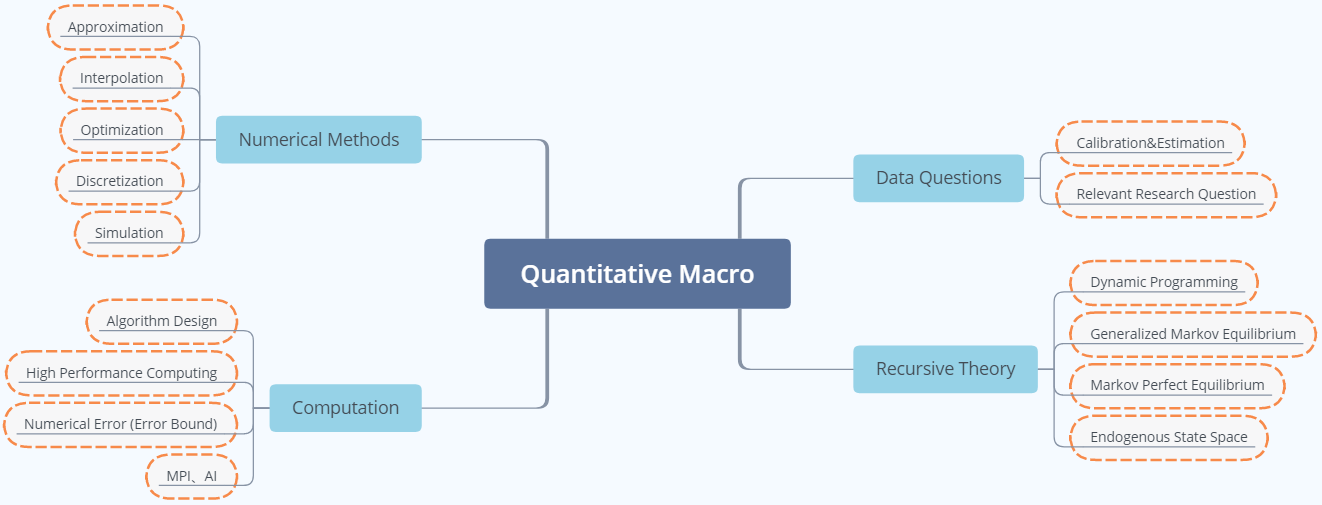
\includegraphics[width=12cm,height=8cm]{pic/quant}
\par\end{center}
\end{frame}

\begin{frame}{Workhorse Models in Quantitative Macro}
\begin{itemize}
\item \textbf{Representative Agent Models:}
\begin{itemize}
    \item Neoclassical (stochastic) optimal growth model
    \item Real Business Cycle (RBC) model
    \item New Keynesian DSGE model
\end{itemize}

\medskip
\item \textbf{Heterogeneous Agent Models:}
\begin{itemize}
    \item Bewley-Aiyagari-Huggett (incomplete markets, idiosyncratic risk)
    \item Krusell-Smith (aggregate uncertainty + heterogeneity)
    \item Overlapping generations (OLG) models
\end{itemize}

\medskip
\item \textbf{Optimal Policy Models:}
\begin{itemize}
    \item Ramsey taxation problems
    \item Time-inconsistency and commitment
\end{itemize}

\medskip
\item \textbf{Common Thread:} All require solving dynamic optimization problems---the Bellman equation is central.
\end{itemize}
\end{frame}

\begin{frame}{Optimal Growth Model at the Core}
\begin{center}
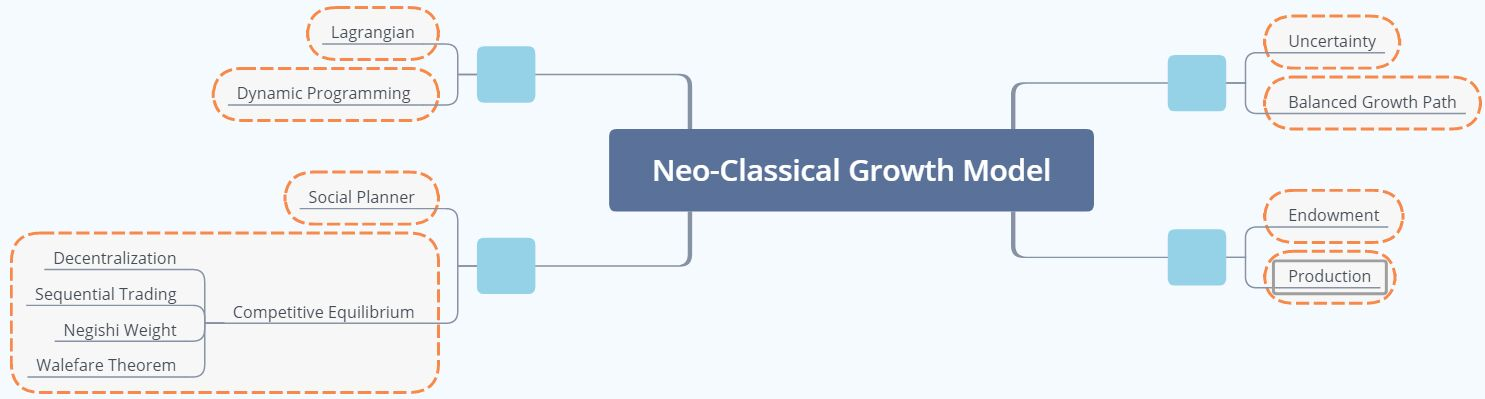
\includegraphics[width=12cm,height=8cm]{pic/neocextension}
\par\end{center}
\end{frame}

\begin{frame}{Optimal Growth Model: Setup}
\begin{itemize}
\item The household solves the following dynamic optimization problem:
\begin{gather*}
\max_{\left\{ c_{t},k_{t+1}\right\} _{t=0}^{\infty}}\sum_{t=0}^{\infty}\beta^{t}\log c_{t} \\
\text{s.t. } c_{t}+k_{t+1}=Ak_{t}^{\alpha}+(1-\delta)k_{t}
\end{gather*}
\[
\beta\in(0,1),\quad A>0,\quad \alpha\in(0,1),\quad \delta\in[0,1]
\]
\[
k_{t}, c_{t}\geq0,\quad k_{0}\text{ given}, \quad t=0,1,2,\dots
\]
\item \textbf{Recursive Formulation (Bellman Equation):}
\[
v(k)=\max_{k' \in \Gamma(k)}\left\{ \log\left(Ak^{\alpha}+(1-\delta)k - k'\right)+\beta v(k') \right\}
\]
where $\Gamma(k) := \left\{ k' \mid 0 \leq k' \leq Ak^{\alpha}+(1-\delta)k \right\}$
\item \textbf{Solution:} Value function $v(k)$ and policy function $k'=g(k)$.
\end{itemize}
\end{frame}

\begin{frame}{From Sequence Problem to Recursive Problem}
\begin{itemize}
\item \textbf{The Challenge:} The sequence problem requires choosing an infinite sequence $\{c_t, k_{t+1}\}_{t=0}^{\infty}$ simultaneously---computationally intractable.

\medskip
\item \textbf{Key Insight:} The problem has \emph{recursive structure}---optimal decisions depend only on the current state $k$, not on history or calendar time.

\medskip
\item \textbf{Bellman's Principle of Optimality (1957):}
\begin{quote}
``An optimal policy has the property that whatever the initial state and initial decision are, the remaining decisions must constitute an optimal policy with regard to the state resulting from the first decision.''
\end{quote}

\medskip
\item \textbf{Implication:} Replace infinite-dimensional optimization with a functional equation---the Bellman equation---reducing the problem to finding a fixed point in function space.
\end{itemize}
\end{frame}

%=============================================================================
\section{Dynamic Programming Foundations}

\begin{frame}{The Bellman Operator}
\begin{itemize}
\item Define the \textbf{Bellman operator} $T: \mathcal{C}(X) \to \mathcal{C}(X)$:
\[
(Tv)(k) = \max_{k' \in \Gamma(k)}\left\{ u\left(Ak^{\alpha}+(1-\delta)k - k'\right)+\beta v(k') \right\}
\]

\medskip
\item The value function $v^*$ is a \textbf{fixed point}: $Tv^* = v^*$

\medskip
\item \textbf{Central Questions:}
\begin{enumerate}
    \item Does a fixed point exist?
    \item Is it unique?
    \item Can we compute it via iteration $v_{n+1} = Tv_n$?
    \item What properties does $v^*$ inherit (continuity, concavity)?
\end{enumerate}

\medskip
\item The following theoretical results answer these questions affirmatively.
\end{itemize}
\end{frame}

\begin{frame}{Contraction Mapping Theorem}
\begin{itemize}
\item \textbf{Definition:} Let $(S, d)$ be a metric space. An operator $T: S \to S$ is a \emph{contraction} with modulus $\beta \in (0,1)$ if:
\[
d(Tv, Tw) \leq \beta \cdot d(v, w) \quad \forall\, v, w \in S
\]

\medskip
\item \textbf{Contraction Mapping Theorem (Banach, 1922):} If $(S,d)$ is a complete metric space and $T$ is a contraction, then:
\begin{enumerate}
    \item $T$ has a \emph{unique} fixed point $v^* \in S$
    \item For any $v_0 \in S$, the sequence $v_{n+1} = Tv_n$ converges to $v^*$
    \item Rate of convergence: $d(v_n, v^*) \leq \frac{\beta^n}{1-\beta} d(v_1, v_0)$
\end{enumerate}

\medskip
\item \textbf{For Economics:} Guarantees that Value Function Iteration (VFI) converges to the unique solution of the Bellman equation.
\end{itemize}
\end{frame}

\begin{frame}{Blackwell's Sufficient Conditions}
\begin{itemize}
\item \textbf{Problem:} How do we verify that $T$ is a contraction?

\medskip
\item \textbf{Blackwell (1965):} An operator $T: \mathcal{B}(X) \to \mathcal{B}(X)$ on bounded functions is a contraction if:
\begin{enumerate}
    \item \textbf{Monotonicity:} $v(x) \leq w(x)$ for all $x$ $\Rightarrow$ $(Tv)(x) \leq (Tw)(x)$
    \item \textbf{Discounting:} $\exists\, \beta \in (0,1)$ such that $T(v + a)(x) \leq (Tv)(x) + \beta a$ for all $a \geq 0$
\end{enumerate}

\medskip
\item \textbf{Verification for the Bellman Operator:}
\begin{itemize}
    \item Monotonicity: Higher continuation value $\Rightarrow$ higher current value
    \item Discounting: The factor $\beta$ in $\beta v(k')$ provides the discounting
\end{itemize}

\medskip
\item \textbf{Key Insight:} The discount factor $\beta < 1$ is not just economically meaningful---it is mathematically essential for convergence.
\end{itemize}
\end{frame}

\begin{frame}{Theorem of the Maximum}
\begin{itemize}
\item \textbf{Theorem (Berge, 1963):} (1963 English translation; original French 1959.) Let $f(x, a)$ be continuous and $\Gamma(x)$ be a continuous, compact-valued correspondence. Then:
\begin{enumerate}
    \item The \emph{value function} $v^*(x) = \max_{a \in \Gamma(x)} f(x,a)$ is continuous
    \item The \emph{policy correspondence} $G(x) = \arg\max_{a \in \Gamma(x)} f(x,a)$ is upper hemi-continuous
\end{enumerate}

\medskip
\item \textbf{Economic Implications:}
\begin{itemize}
    \item Small changes in $k$ lead to small changes in $v(k)$ and $g(k)$
    \item Ensures stability of computed solutions
    \item Justifies numerical approximation on discrete grids
\end{itemize}

\medskip
\item \textbf{Additional Properties:} Under strict concavity of $u(\cdot)$ \emph{and} a convex constraint graph (i.e.\ $\Gamma$ has convex graph, so the feasible set is convex):
\begin{itemize}
    \item Policy correspondence is single-valued: a \emph{function} $g(k)$
    \item Value function $v(k)$ is strictly concave
\end{itemize}
\end{itemize}
\end{frame}

\begin{frame}{Theoretical Foundation: Summary}
\begin{center}
\begin{tabular}{l l}
\toprule
\textbf{Result} & \textbf{What It Guarantees} \\
\midrule
Principle of Optimality & Recursive formulation is valid \\
Contraction Mapping Thm & Existence, uniqueness, convergence \\
Blackwell's Conditions & Easy verification of contraction \\
Theorem of the Maximum & Continuity and stability \\
\bottomrule
\end{tabular}
\end{center}

\bigskip
\textbf{Together, these results establish:}
\begin{enumerate}
    \item The Bellman equation has a \emph{unique} solution $v^*$
    \item We can \emph{compute} $v^*$ by iterating $v_{n+1} = Tv_n$
    \item The solution is \emph{well-behaved} (continuous, concave)
    \item The policy function $g(k)$ is \emph{stable} under perturbations
\end{enumerate}

\bigskip
$\Rightarrow$ \textbf{Solid foundation for computational methods}
\end{frame}

\end{document}
